\section{Kasutajaliides}
Vastavalt peatükile \ref{analysis_interface_subsection} kasutajaliidese realiseerimise tehnoloogiaks
on valitud React.Js raamistik.

Kasutajaliidese rakendus koosneb \textit{React JSX.Element} komponentidest ja teenustest.
Komponendid tagavad rakendusele nõutud funktsionaalsust ja välimust ning teenused vahendavad andmeid komponentide 
ja serveriosa vahel.

Rakenduse koosseisus on palju erinevaid komponente, suureb osa nendest on lihtsamad komponendid või tavalised
CRUD-loogikaga komponendid, mistõttu ei ole nende realiseerimise käesolevas peatükis eraldi kirjeldatud. Koodibaas
täismahus on vaadatav  Lisas X oleva viitega koodi repositooriumile. Käesolevas peatükis kirjeldatakse vaid mõned
komponendid, mis infosüsteemi äriloogika seisukohalt vajavad kompleksset ülesehitust ja funktsionaalsust -- 
ehitusmaterjali lisamise vorm ja kalkulaator.

Materjali loomiseks ja redigeerimiseks on luuakse vorm, mis täidab samaaegselt mõlemat rolli.
Kui vormi avamisel oli antud ehitusmaterjali ID, siis laetakse vastav materjal andmebaasist redigeerimiseks, 
vastasel juhul vormi avamisel luuakse serveriosale päringuga uus materjal mustandi staatusega, mida hakatakse
vormis redigeerima. Materjali vorm koosneb kahest React komponendist - vormi põhi ja materjali omaduse plokk.
Vormi põhi on suurem komponent \textit{MaterialForm.tsx}, mille kaudu redigeeritakse materjali staatilised 
väljad:

\begin{itemize}
    \item nimetus (\textit{title}) -- tekstiväli,
    \item materjali tüüp (\textit{materialCategoryId}) -- valiklist materjalide kategooriatest, 
    \item tootja (\textit{manufacturerId}) -- valiklist materjalide tootjatest,
    \item allikas (\textit{source}) -- tekstiväli,
    \item viide allikale (\textit{link}) -- tekstiväli,
    \item kommentaar (\textit{comment}) -- tekstiväli.
\end{itemize}

Materjalide omaduste (nt tihedus, soojusjuhtivus) arv on muutuv -- mõne materjali puhul võivad olla salvestatud
kõik omadused, teise materjali puhul vaid mõned neist. Lisaks sellele, tulevikus võib infosüsteemile olla lisatud
võimalus salvestada muud omadused, mis on tarvis teiste arvutuste jaoks. Sellest tingituna peab olema võimalus kuvada
ja redigeerida need omadused, mis on materjali puhul määratud. Lisaks peavad olema näidatud ka omadused,
mida on võimalik lisaks määrata. Materjali omadusi redigeerimiseks tehakse väiksem taaskasutatav 
komponent \textit{MaterialPropertyCard.tsx}. Komponendil on järgmised väljad:
\begin{itemize}
    \item väärtus (\textit{value}) -- materjali omaduse arvuline väärtus,
    \item tõendatud (\textit{verified}) -- boolean väärtus,
    \item allikas (\textit{source}) -- tekstiväli.
\end{itemize}

Põhikomponendis on redigeeritava materjali puhul eksisteerivad omadused on salvestatud vormi oleku objektis \textit{materjal.materialProperties}
listi kujul. Iga omaduse jaoks luuakse iteratiivselt vastav komponent \textit{MaterialPropertyCard}, millele antakse omaduse objekt ja funktsioon, 
mis töötleb sisendi andmete muutmist ja tagastab põhikomponendisse sisestatud väärtused. Põhikomponendis uuendatakse olekut ja vastavalt
saadetakse ka päringuid materjali uuendamiseks andmebaasis. Komponendil \textit{MaterialPropertyCard} välimuse seisukohalt on kaks olekut sõltuvalt 
sellest, kas 
\begin{itemize}
    \item vastav omadus on materjalile lisatud
    \item vastav omadus ei ole materjalile lisatud, kuid seda on võimalik lisada.  
\end{itemize}

Materiali omaduste komponentide välimus mõlemas olekus on näidatud pildil \ref{fig:development_frontend_propertycard}.
 \begin{figure}[ht]
    \centering
    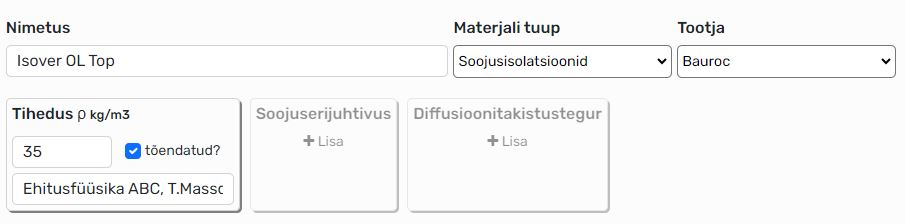
\includegraphics[width=1\textwidth]{figures/development/frontend_propertycard.JPG}
    \caption[\textit{PropertyCard} materjali omaduste komponendid materjali vormis]{\textit{PropertyCard.tsx komponendid materjali vormis}}
    \label{fig:development_frontend_propertycard}
\end{figure}

Infosüsteemi teine oluline ning keerulisema loogikaga osa on kalkulaator. Kalkulaator koosneb järgmistest plokkidest:
\begin{itemize}
    \item arvutuse seadistuste osa, milles valitakse arvutuse parameetrid (sise- ja välis keskkond, konstruktsiooni tüüp);
    \item konstruktsiooni kihtide plokk, milles lisatakse konstruktsioonile kihte ja valitakse kihtide omadused (materjal, paksus);
    \item tulemuste esitamise plokk, milles graafiliselt esitatakse konstruktsiooni kihtide skemaatilist joonist, graafikuid ning arvuline tulemus 
    (soojusjuhtivus U ja veeaurutakistus Zp).
\end{itemize}

Kalkulaatori põhiline \textit{React} komponent on \textit{Therm.tsx}. Komponent juhib ja korraldab alluvate komponentide tööd. Komponendis on mitu oleku (\textit{state}) objeki:
\begin{itemize}
    \item \textit{optionsLibrary} -- objekt, mis hoiab arvutuse parameetrite valikud (keskkonnad, konstruktsioonitüübid),
    \item \textit{materials} -- objekt, mis hoiab materjale, mida kasutatakse konstruktsiooni kihtide mudeldamisel,
    \item \textit{calculationData} -- objekt, mis hoiab arvutuse lähteandmeid, mida edastatakse serverile
    \item \textit{calculationResult} -- objekt, mis hoiab serverilt tulnud arvutuse tulemused.
\end{itemize}

Ülaltoodud objektide loomiseks kasutatakse  sisseehitatud lahendust \textit{UseState}, mille abil loob React juhitavat oleku objekti. \textit{UseState}
objektide eelis on oleku muutuste jälgimine ning kõikide olekust sõltuvate komponentide automaatne uuendamine oleku muutmisel.

Kalkulaatori põhikomponent koosneb väiksematest komponentidest, mis oma funktsionaalsusest lähtuvalt vastavad varem nimetatud kalkulaatori plokidele.
Kalkulaatori alamkomponendid on:
\begin{itemize}
    \item \textit{ThermOptions.tsx} -- komponendile antakse arvutuse parameetrite andmeobjekt, arvutuse lähteandete objekt ning funktsioon kasutajasisendi töötluseks;
    sisendi muutmisel tagastab komponent põhikomponendisse sisendi uut väärtust, millega uuendatakse arvutuse lähteandmete objekti.
    \item \textit{LayersBlock.tsx} -- komponendile antakse edasi ehitusmaterialide andmeobjekt, mida kasutatakse konstruktsiooni kihtide lisamise vormis, ning funktsiooni
    konstruktsiooni kihtide salvestamiseks; komponent on kompleksse ülesehitusega ja omakorda omab struktuuris alamkomponente; komponent tagastab põhikomponendisse konstruktsiooni
    kihtide listi;
    \item \textit{ResultBlock.tsx} -- komponendile antakse kihtide plokis koostatud kihtide objekt ning serverilt tulnud arvutuse tulemused graafikute joonestamiseks. 
\end{itemize}

\textit{Therm.tsx} komponendi struktuur on toodud Pildil \ref{fig:development_frontend_therm}.
\begin{figure}[ht]
    \centering
    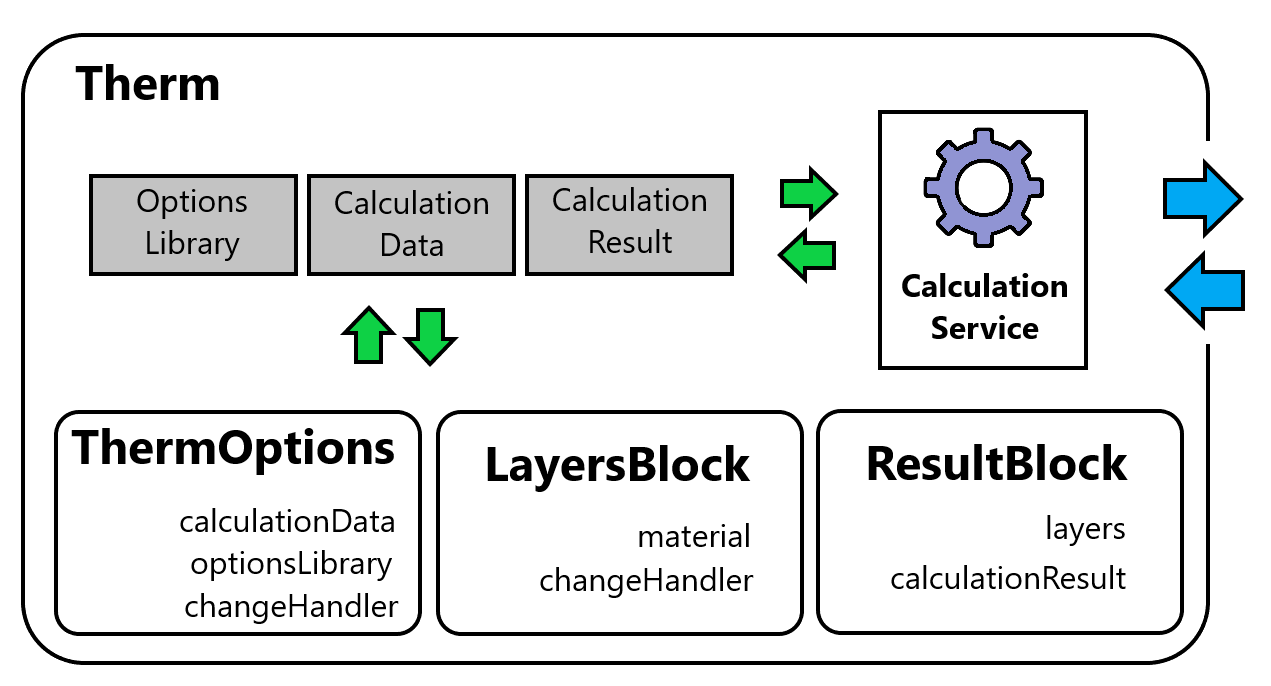
\includegraphics[width=1\textwidth]{figures/development/frontend_term_structure.png}
    \caption[Kasutajaliidese komponendi \textit{Therm.tsx} struktuur]{\textit{Therm.tsx komponendi struktuur}}
    \label{fig:development_frontend_therm}
\end{figure}

Alamkomponentide loogika on piiratud oma vastutusalaga, kõik alamkomponendid on üks teisest sõltumatud ning on juhitud põhikomponendist. Serveriosaga suhtlemine toimub põhikomponendis
oleva teenuse kaudu (\textit{CalculationService}). Põhikomponent küsib teenuse kaudu serveriosalt andmeid, mis on tarvis kalkulaatoris olevate valiklistide täitmiseks ja komplekteerib
kasutajas isendist andmeobjekti, mille struktuur vastab vastab serveriosa vastavale liidesele. Samuti komponent saadab serverile päringut arvutuse lähteandmetega ning 
töötleb ja edastab vastust tulemuste esitamise komponendile.
